\subsection{Relational databases}
The group last year chose to implement the \texttt{WordCount} (see Section \ref{sec:Sprint2And3}) and \texttt{Fuseki} databases using PostgreSQL.
Postgres is a relational database system \cite{knox2020}.


A relational database consists of several layers.
The lowest level is the physical layer which describes how the data are stored physically.
The purpose of the relational model is to abstract over the physical layer of the database.
This abstraction is known as the logical layer and allows database administrators to manage the physical storage without directly manipulating the physical data representation.
The logical layer describes what data are stored and the relationships between the data.
The highest of abstraction is the view layer which describes only part of the database. It exists to simplify the interaction with the system. Many views may exist for the same database.
\cite[Chapter 1.3]{DBSBook}

Compared to storing data on a regular file system, a database system provides many advantages including atomicity of operations, concurrent access to data, and lowered inconsistency and redundancy of data \cite[Chapter 1.2]{DBSBook}.
These advantages can be directly seen in the ACID properties that databases adhere to when performing a transaction (see Section \ref{sec:SQL}) \cite[Chapter~17]{DBSBook}.
\begin{itemize} \label{ACID}
    \item Atomicity: A transaction must either be fully completed or partial side-effects of a failed transaction must be undone.
    \item Consistency: A transaction in isolation must ensure values remain consistent after a transaction has been completed or terminated.
    \item Isolation: Transactions are unaware of other transactions being executed concurrently to avoid confusion.
    \item Durability: Changes caused by a committed transaction persist even in the event of system failures.
\end{itemize}

In the coming sections, we will describe how one can model and describe a relational database design, both mathematically and with a more graphic design.
After doing this, we will examine how operations on these models can be described using SQL (Section~\ref{sec:SQL}) and relational algebra (Section~\ref{sec:relationalAlgebra}).

\subsubsection*{Relational model}
Relational database systems can be mathematically described using relations and sets, mapping a unique key to a tuple of information \cite[Chapter~2.3]{DBSBook}.
The values of the tuples contained within the relation can be described by the attributes of the relation and their corresponding domains \cite{KatjaFirstPP}. 
The relations are often described using a \textit{relational schema}, denoting the name and domains of the attributes.


Equation \ref{eq:relational_schema} shows an example of a relation describing books as quadruples of three text fields (author\_name, title, and ISBN) and a positive integer (number\_of\_pages).
The relation also denotes a super key for the relation. A super key is one or more attributes that can uniquely identify a tuple in a given relation. Attributes describing the super key are underlined.

\begin{equation} \label{eq:relational_schema}
    book(author\_name:text, title: text, number\_of\_pages:\mathbb{Z}^+, \underline{ISBN: text})
\end{equation}
Super keys can be defined as $t_1 \in r,\neq t_2 \in r \implies t_1.K \neq t_2.K$. 

That is, no two tuples $t_1, t_2$ from relation $r$ have same values for all super key attributes $K$. 
If the super key does not contain extraneous attributes, it is said to be \textit{minimal}. \cite[Chapter 2.3]{DBSBook}
We will use the term \textit{primary key} to denote a chosen super key of a relation. 
When describing a database, it is often necessary to specify how various data are connected. 
To do this, one can use \textit{foreign keys} to denote that tuples in $r_1$ are related to the tuples in $r_2$.


One could model the relationship between a book owner and a book using the relational schemas seen in equation \ref{eq:bookOwnerExample} and \ref{eq:relational_schema}.
There, primary keys from other relations are used to reference unique tuples. The $owns$ relation describes how relations $book$ and $book\_owner$ are connected. 
\begin{equation}\label{eq:bookOwnerExample}
    \begin{split}
        owns(\underline{owner\_id \rightarrow book\_owner}, \underline{ISBN \rightarrow book}), \\
        book\_owner(name:text,\underline{owner\_id:\mathbb{Z}^+})
    \end{split}
\end{equation}

Instead of describing the data structures of the database in these relations, one can use a different model that represents the logic of the relational schemas.

\subsubsection{Entity relation model}\label{sec:EntityRelationModel}
The entity relation model is a graphical representation of how database relations are structured.
This is done in a \textit{E-R diagram}, and is commonly used facilitate database design from specifications of enterprise schemas \cite*[Chapter 6.2]{DBSBook}.
However, in the E-R model we differentiate between \textit{relationships sets} connecting relations and \textit{entity sets} representing domain elements. 
The entity sets are represented graphically with a rectangle and relationship sets connecting the entity sets with a diamond \cite[Chapter 6.2]{DBSBook}.
The attributes associated with the entity- and relationship sets can be modelled using ovals \cite{KatjaFirstPP}, however other alternatives exists.\footnote{Our style of choice is presented in Chapter 6.10 of \citetitle{DBSBook} \textit{\citefield[]{DBSBook}[]{edition}}}
Similar to the relational model, the entities (tuples) must be uniquely identified by one or more attributes. This is denoted by underlining the attributes. 

The E-R model have notations that denotes the participations each entity have in a connecting relationship \cite[Chapter 6.4]{DBSBook}.
In this project, we will use \text{min-max} notation; this notation denotes the minimum and maximum amount of entities participating in a relationship. 

\begin{figure}[htp]
    \centering
    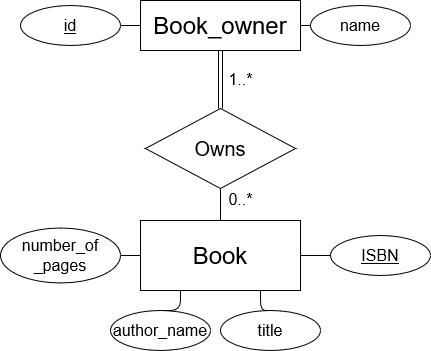
\includegraphics[scale=0.5]{Images/book_example_w_cardinality.png}
    \caption{E-R diagram of the book and book owner example.}
    \label{fig:ER_Book_Example}
\end{figure}

Figure \ref{fig:ER_Book_Example} shows the $book$, $owns$, and $book_owner$ relations from equation \ref{eq:bookOwnerExample} and \ref{eq:relational_schema}.
In figure \ref{fig:ER_Book_Example} we also see the  the participation cardinalities of the two entity sets. 
The relationship from $book\_owner$ to $owns$ is a one-to-many relationship. That is, each book owner entity must own at least one book. Thus the relationship has total participation. 
\begin{figure}[h]
    \centering
    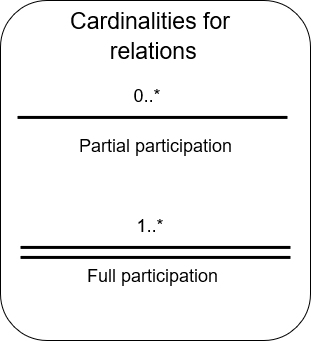
\includegraphics[scale=0.5]{Images/cardinalities.png}
    \caption{Participation ratios for ER relationships}
    \label{fig:ERDiagram_Cardinality}
\end{figure}
The relationship from $book$ to $owns$ is zero-to-many. That is, the diagram represents books that no one owns, and that a book can be owned by multiple book owners.
This relationship does not have total participation. Participation connections can be seen on figure \ref{fig:ERDiagram_Cardinality}.


Other forms of entity sets exits. For instance, a weak entity set, denoted by a an oval with doubled edges, is an entity sets whose existence is based on another entity set.
A weak entity set is identified by its \textit{identifying entity set}'s primary key along with extra attributes. 
The relationship between weak entity sets and its identifying set is always many-to-one with total  participation of the weak entity set.

Since the relational model is described using sets, we can also describe operations that can be performed on the relations.
Therefore, it is useful to be able to convert an E-R model into an equivalent relational model, where domains of attributes can be well defined and operations on the entity sets described mathematically.

\subsubsection*{Converting E-R models to relations}
When converting non-weak entity sets to relations, one create a relation with a primary key attribute with the same name of the primary key of the entity set \cite[Chapter 6.7.1]{DBSBook}.
The remaining attributes of the entity set is similarly mapped to the relation. 

When representing weak entity sets, one creates a relation containing the attributes of the weak entity set as well as the attributes of the identifying set's primary keys. 
The primary key of the relation will consist of the identifying sets primary keys and the weak entity sets primary keys. 
The primary key of the identifying relation will also serve as a foreign key to the identifying relation.  \cite[Chapter 6.7.1]{DBSBook}.

E-R relationship sets are converted to relations by forming a union of all primary keys of the participating entity sets, along with any attributes of the relationship set. 
The primary keys for the participating entity sets are used as a foreign keys to their corresponding relation.
If the relationship is between a weak- and its identifying entity set, it is simply ignored, as the relationship set will not have any attributes, and the relation created from the weak entity will already have a foreign key referencing the identifying entity \cite[Chapter 6.7.5]{DBSBook}. 

If we have a many-to-one relationship between two sets, with total participation on the 'many' side, we can combine the relationship and the relation created from the 'many' side and the relationship.
This new schema will have use the primary key of the entity set as its primary key.
When converting one-to-one relationships, we simply create a union of the attributes from the relationship and the two relationship sets. \cite*[Chapter 6.7.6]{DBSBook}

\subsubsection{Relational algebra}\label{sec:relationalAlgebra}
Relational algebra describes a set of unary and binary operations on relations that produce new relations.
The operations are used to define new relations, often the tuples within the set will satisfy defined predicates.
The relational operators form the foundations of data manipulation languages (see Section \ref{sec:SQL}) which can be used to define database operations \cite[Chapter 6.2]{DBSBook}.


\begin{table}[h]
    \centering
    \begin{tabular}{|lll|}
    \hline 
    \multicolumn{1}{|l|}{\textbf{Operator}}          & \multicolumn{1}{l|}{\textbf{Example}}   & \multicolumn{1}{l|}{\textbf{Is unary}}      \\ \hline
    \multicolumn{1}{|l|}{Select}                     & \multicolumn{1}{l|}{$\sigma_{predicate}(R)$}             & \multicolumn{1}{l|}{$\checkmark$}           \\ \hline
    \multicolumn{1}{|l|}{Projection}                 & \multicolumn{1}{l|}{$\pi_{A_1, A2,...,A_n}(R)$}             & \multicolumn{1}{l|}{$\checkmark$}           \\ \hline
    \multicolumn{1}{|l|}{Join}                 & \multicolumn{1}{l|}{$r_1 \Join_\Theta r_2$}             & \multicolumn{1}{l|}{$\times$}           \\ \hline
    \multicolumn{1}{|l|}{Cartesian product}          & \multicolumn{1}{l|}{$r_1\times r_2$}              & \multicolumn{1}{l|}{$\times$}            \\ \hline
    \end{tabular}
    \caption{Table of operators}
    \label{Relational algebra operators}
\end{table}

We will describe some of the operators of relational algebra, and use them to describe implemented queries later.
Some of the common operators of in relational algebra can be seen on table \ref{Relational algebra operators}.\\
\textbf{Select}\\
The select operator defines a set, $R_{result}\subseteq R$ where all tuples $t \in R_{result}$ satisfies a given predicate \cite[Chapter 2.6.1]{DBSBook}.\\
That is, $\forall t \in R_{result} \vDash predicate$.\\
\textbf{Projection}\\
The projection operator specifies a relation containing only a subset of the attributes of the operand relation \cite[Chapter 2.6.2]{DBSBook}.
That is, attributes $A_1, ..., A_n$ of relation $R_{result}$ will be a subset or equal to the attributes of the operand.\\
\textbf{Cartesian product}\\
The cartesian product of two relations $R_1$ and $R_2$ produces a set containing concatenated tuples of the two operands.
That is, taking the attributes of the two sets, $A_1,...,A_n \in R_1$ and $A_{n+1},...,A_k \in R_2$ produces a set with attributes $A_1,...,A_k$.
If the attributes of the operands have the same names we distinguish between them  by denoting their original relation: $R_1.AttributeName$, $R_2.AttributeName$. \cite[Chapter 2.6.4]{DBSBook}\\   
\textbf{Join}\\
The join operator defines a relation consisting of tuples from the cartesian product of the operand, containing only tuples satisfying the given predicate.
Thus it is defined as $\sigma_{\Theta} (R_1 \times R_2)$ \cite[Chapter 2.6.5]{DBSBook}.

As we have now established both how to model database relations as well fundamental operations used to extract data (tuples) from these relations, we can now look at how to implement the relations in a database.

\subsubsection{SQL}\label{sec:SQL}
-> What is SQL
-> What is DDL
-> What is DML
   --> How is it similar to relational algebra?
Data from a relational database can be queried using relational query languages such as SQL.
Executing a query instructs the database system to perform a set of operations to compute a desired result. Collectively, the resulting set of operations is known as a transaction.

Having established how one can define a database schemas using SQL as a DLL, as well as query data from the database using SQL as a DML, we will now discuss how one can evaluate a database design.
\subsubsection*{Evaluating a database design}
